\documentclass [12pt] {article}
\textheight=8.0in
\textwidth=8.0in
\topmargin=-1.0in
\raggedbottom
\oddsidemargin=-2.0cm
\evensidemargin=2.0cm
\usepackage{latexsym}
\usepackage{graphicx}
\usepackage{fancyhdr}
\usepackage{longtable}
\usepackage[table]{xcolor}
\usepackage{eso-pic}
\usepackage{afterpage}
\usepackage{lastpage}
\usepackage{csvsimple}
\usepackage{datetime}
\usepackage{pgffor}
\usepackage{underscore}
\usepackage{hyperref}
\usepackage{vwcol}
%\usepackage[francais]{babel}
\usepackage[T1]{fontenc}
\usepackage[utf8]{inputenc}
\usepackage{etoolbox}

\renewcommand{\headheight}{1.0in}
\renewcommand{\headrulewidth}{2pt}
\renewcommand{\footrulewidth}{1pt}
\setlength{\headwidth}{\textwidth}
\setlength{\LTpre}{-10pt}

\pagestyle{fancy}

\definecolor{light-gray}{gray}{0.95}
\definecolor{dark-gray}{gray}{0.8}
\definecolor{light-blue}{rgb}{0,0,0.99}
\definecolor{babyblueeyes}{rgb}{0.63, 0.79, 0.95}


% To speed up the compilation time, use a precompiled preamble
%\endofdump % End of static part. The precompiled preamble will contain everything above this line


%\fancyhead[L]{\large\textbf{Patient-Reported Outcomes Report}}
\fancyhead[C]{
\includegraphics[height=0.53in]{src/QIP/Resources/latex-markup/images/logo.png}\\}

\fancyhead[L]{\large\textbf{Questionnaires remplis et déclarés par le patient}}

\fancyhead[R]{\large\textbf{\patientName\\\patientMRN}}  % \\ \today\ \currenttime

\fancyfoot[R]{Page \thepage~de ~\pageref*{LastPage}} %page number on right
\fancyfoot[C]{} %blank central footer
\lfoot{\textbf{FMU-8624 Source :} ARIA(REV 2018/08/24) \\
\hfill\\
\footnotesize{Si une version papier de ce document est re\c{c}ue aux archives, avec ou sans notes manuscrites, en statut pr\'{e}liminaire ou final, \textbf{il ne sera pas num\'{e}ris\'{e}}.  Les corrections doivent \^{e}tre faites dans le document pr\'{e}liminaire ou via l'addendum si le document est final.\\
\hfill\\
If a printout of this document is received in Medical Records, with or without handwritten notes, whether it is preliminary or final, \\textbf{it will not be scanned}.  Corrections must be done in the preliminary document or via an addendum if the document is final.}
}

\def\addtablerow#1/#2!{#2 & #1\\ \hline}

\newcommand{\myTable}[2]{
\renewcommand*\do[1]{\addtablerow##1!}

    \begin{longtable}
    {
    |p{0.17\linewidth}
    |p{0.4\linewidth}
    |
    }

    \rowcolor{white}\multicolumn{1}{l}{\color{white}{ }}\\
    \hiderowcolors
    \caption*{\large Question: #2}\\
    \showrowcolors
    \hline
    \rowcolor{babyblueeyes}
    \textbf{Date} %completed questionnaired
    &\textbf{Response} %last updated
    \\ \hline
    \endhead
    \hline
    \hline

    \docsvlist{#1}
    \hline
    \end{longtable}
}


\begin{document}

\normalsize
\rowcolors{1}{light-gray}{dark-gray}
\begin{minipage}{.45\linewidth}
    \begin{flushleft}
        \hspace{60pt} \textbf{\Large \patientName} \\
        \hspace*{60pt} \textbf{\Large \patientMRN}
    \end{flushleft}
\end{minipage}
\hfill
\begin{minipage}{.60\linewidth}
     \hspace{120pt} 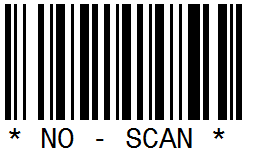
\includegraphics[height=0.8in]{src/QIP/Resources/latex-markup/images/noscan.png}
\end{minipage}

%\begin{flushleft}
%    \textbf{\Large \patientName} \\
%    \textbf{\Large \patientMRN} \\
%\end{flushleft}

%\shorthandoff{:}

{\renewcommand{\arraystretch}{1.5}%row padding
\begin{longtable}
{
|p{0.4\linewidth}
|p{0.2\linewidth}
|p{0.05\linewidth}
|
}
    \rowcolor{white}\multicolumn{1}{l}{\color{white}{ }}\\
    \hline
    \rowcolor{babyblueeyes}
    \textbf{Questionnaires rempli} %completed questionnaired
    &\textbf{Dernière mise à jour} %last updated
    &\textbf{Page}
    \\ \hline
    \endhead
    \hline
    \hline

    \csvreader[head to column names, late after line=\\\hline]{\csvContentTablePath}{}% use head of csv as column names
    {\hyperlink{\questionnaireID}{\questionnaireNickname} & \lastUpdated & ~\pageref*{\questionnaireID}}
    % specify your coloumns here
\end{longtable}

}

\foreach \patientId/\timestamp/\lastUpdated/\questionnaireNickname/\questionnaireID/\imagesFolder/\imagesArray/\textQuestions/\textQuestionsArray in \imageDirectories{%
    \newpage

    \begin{center}
        \hypertarget{\questionnaireID}{}
        \label{\questionnaireID}
        ~\ref{\questionnaireID}
        \large\textbf{\questionnaireNickname}\\
        \large\textbf{Dernière mise à jour: \lastUpdated \\ } %last updated
    \end{center}

    \foreach \imageID in \imagesArray {
        \begin{center}
            \includegraphics[height=18.0cm, width=14.0cm]{./built-chart-images/\patientId/\timestamp/\imagesFolder/\questionnaireID/\imageID}
        \end{center}
    }

   \ifdefempty{\textQuestionsArray}{}{
       \foreach \textQuestion/\answersArray in \textQuestionsArray {
           \expandafter\myTable\expandafter{\answersArray}{\textQuestion}
       }
   }
}

\end{document}